\documentclass[tikz,border=5pt]{standalone}
\usepackage{tikz}

\begin{document}
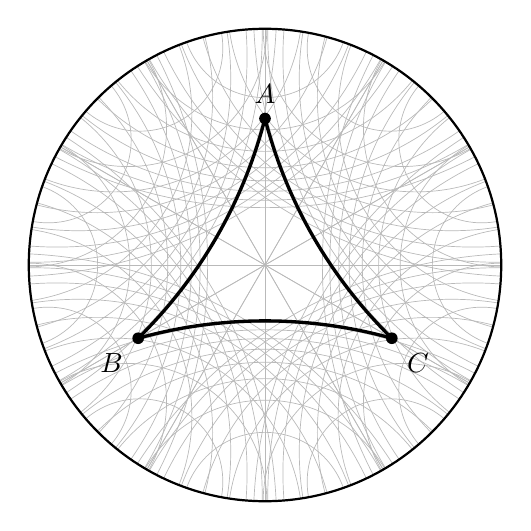
\begin{tikzpicture}[scale=3, line cap=round, line join=round]

  % Styles
  \tikzset{
    grid/.style={line width=0.25pt, gray!55},
    tri/.style={very thick}
  }

  % --- Geodesic grid (behind) ---
  \begin{scope}
    \clip (0,0) circle (1);

    % Radial geodesics (diameters) every 30�
    \foreach \k in {0,...,11} {
      \pgfmathsetmacro{\ang}{30*\k}
      \draw[grid] ({cos(\ang)},{sin(\ang)}) -- ({-cos(\ang)},{-sin(\ang)});
    }

    % Families of geodesic arcs: circles orthogonal to the boundary
    % Centers at distance a>1 from origin; radius R = sqrt(a^2-1); rotate every 30�
    \foreach \a in {1.06,1.16,1.28,1.42,1.58,1.76,1.96,2.18} {
      \pgfmathsetmacro{\R}{sqrt(\a*\a - 1)}
      \foreach \k in {0,...,11} {
        \pgfmathsetmacro{\ang}{30*\k}
        \draw[grid] ({\a*cos(\ang)},{\a*sin(\ang)}) circle (\R);
      }
    }
  \end{scope}

  % Boundary of the Poincar� disk
  \draw[thick] (0,0) circle (1);

  % --- Symmetric triangle: three points at same radius, 120� apart ---
  \pgfmathsetmacro{\r}{0.62}
  \pgfmathsetmacro{\aA}{ 90}
  \pgfmathsetmacro{\aB}{210}
  \pgfmathsetmacro{\aC}{330}
  \pgfmathsetmacro{\Ax}{\r*cos(\aA)} \pgfmathsetmacro{\Ay}{\r*sin(\aA)}
  \pgfmathsetmacro{\Bx}{\r*cos(\aB)} \pgfmathsetmacro{\By}{\r*sin(\aB)}
  \pgfmathsetmacro{\Cx}{\r*cos(\aC)} \pgfmathsetmacro{\Cy}{\r*sin(\aC)}

  % Hyperbolic geodesic (Poincar� disk): arc orthogonal to boundary
  \newcommand{\DrawHArc}[4]{%
    \pgfmathsetmacro{\px}{#1} \pgfmathsetmacro{\py}{#2}
    \pgfmathsetmacro{\qx}{#3} \pgfmathsetmacro{\qy}{#4}
    \pgfmathsetmacro{\vx}{\qx - \px}
    \pgfmathsetmacro{\vy}{\qy - \py}
    \pgfmathsetmacro{\vlen}{sqrt(\vx*\vx + \vy*\vy)}
    \ifdim \vlen pt < 0.000001pt
    \else
      \pgfmathsetmacro{\nx}{-\vy/\vlen}
      \pgfmathsetmacro{\ny}{ \vx/\vlen}
      \pgfmathsetmacro{\mx}{(\px+\qx)/2}
      \pgfmathsetmacro{\my}{(\py+\qy)/2}
      \pgfmathsetmacro{\pp}{\px*\px + \py*\py}
      \pgfmathsetmacro{\mp}{\mx*\px + \my*\py}
      \pgfmathsetmacro{\np}{\nx*\px + \ny*\py}
      \pgfmathsetmacro{\abnp}{abs(\np)}
      \ifdim \abnp pt < 0.000001pt
        % Diameter case (straight)
        \draw[tri] (\px,\py) -- (\qx,\qy);
      \else
        % Center c and radius R of the supporting circle
        \pgfmathsetmacro{\tpar}{(1 + \pp - 2*\mp)/(2*\np)}
        \pgfmathsetmacro{\cx}{\mx + \tpar*\nx}
        \pgfmathsetmacro{\cy}{\my + \tpar*\ny}
        \pgfmathsetmacro{\dxp}{\px-\cx}
        \pgfmathsetmacro{\dyp}{\py-\cy}
        \pgfmathsetmacro{\R}{sqrt(\dxp*\dxp + \dyp*\dyp)}
        \pgfmathsetmacro{\tP}{atan2(\py-\cy,\px-\cx)}
        \pgfmathsetmacro{\tQ}{atan2(\qy-\cy,\qx-\cx)}
        \pgfmathsetmacro{\dAng}{mod(\tQ-\tP+540,360)-180}
        % choose the inside arc
        \pgfmathsetmacro{\tMid}{\tP + \dAng/2}
        \pgfmathsetmacro{\rx}{\cx + \R*cos(\tMid)}
        \pgfmathsetmacro{\ry}{\cy + \R*sin(\tMid)}
        \pgfmathsetmacro{\rin}{\rx*\rx + \ry*\ry <= 1 ? 1 : 0}
        \ifnum \rin=0
          \pgfmathsetmacro{\dAng}{\dAng > 0 ? \dAng-360 : \dAng+360}
        \fi
        \pgfmathsetmacro{\tA}{\tP}
        \pgfmathsetmacro{\tB}{\tP+\dAng}
        \pgfmathsetmacro{\ta}{min(\tA,\tB)}
        \pgfmathsetmacro{\tb}{max(\tA,\tB)}
        \draw[tri]
          plot[domain=\ta:\tb, samples=140, variable=\t]
            ({\cx + \R*cos(\t)}, {\cy + \R*sin(\t)});
      \fi
    \fi
  }

  % Geodesic triangle
  \DrawHArc{\Ax}{\Ay}{\Bx}{\By}
  \DrawHArc{\Bx}{\By}{\Cx}{\Cy}
  \DrawHArc{\Cx}{\Cy}{\Ax}{\Ay}

  % Vertices
  \fill (\Ax,\Ay) circle (0.7pt) node[above=2pt] {$A$};
  \fill (\Bx,\By) circle (0.7pt) node[below left=2pt] {$B$};
  \fill (\Cx,\Cy) circle (0.7pt) node[below right=2pt] {$C$};

\end{tikzpicture}
\end{document}
